% Chapter 5

\chapter{Evaluation of the Model} % Main chapter title

\label{Chapter5} % For referencing the chapter elsewhere, use \ref{Chapter5}

% This is for the header on each page - perhaps a shortened title
\lhead{Chapter 5. \emph{Evaluation of the Model}}

% Quotation
``Science, my boy, is made up of mistakes, but they are mistakes which it is useful to make,because
they lead little by little to the truth"

\begin{flushright}
Jules Verne, \textit{Journey to the Centre of the Earth} (1864)
\end{flushright}

%---------------------------------------------------------------------------------------------------
%	CONTENT
%---------------------------------------------------------------------------------------------------

\section{Experimental setup}
% Brunswick Road - 6336, 6338; 16572
% Flemington Road - 3393, 3394, 3396, 3398; 13632, 13634, 13635, 13637
% Elizabeth Street -
% Victorial Parade - 3592, 3593, 3594, 3595, 3596; 13829, 13831, 13832, 13835
% Hoddle Street - 268, 272, 273, 274, 275, 277, 278; 6278, 10522, 10523, 10525, 10526, 10527, 10528, 16515, 16517
% Nicholson Street - 5539, 5540, 5541, 5543, 5544, 5545, 9615; 15773, 15774, 15775, 15777, 15778, 19854, 19855
% Royal Parade - 6782, 6783, 6784, 6786; 17022, 17023, 17025
% Lygon Street - 9424, 9425, 9426, 9427, 9429; 19659, 19660, 19661, 19662, 19663
We chose a subset of the obtained traffic data for experimentation as shown in the figure
\ref{fig:ExperimentRegion}. The region boundary of the subnetwork is denoted by the red line.

\begin{figure}[htbp]
  \centering
    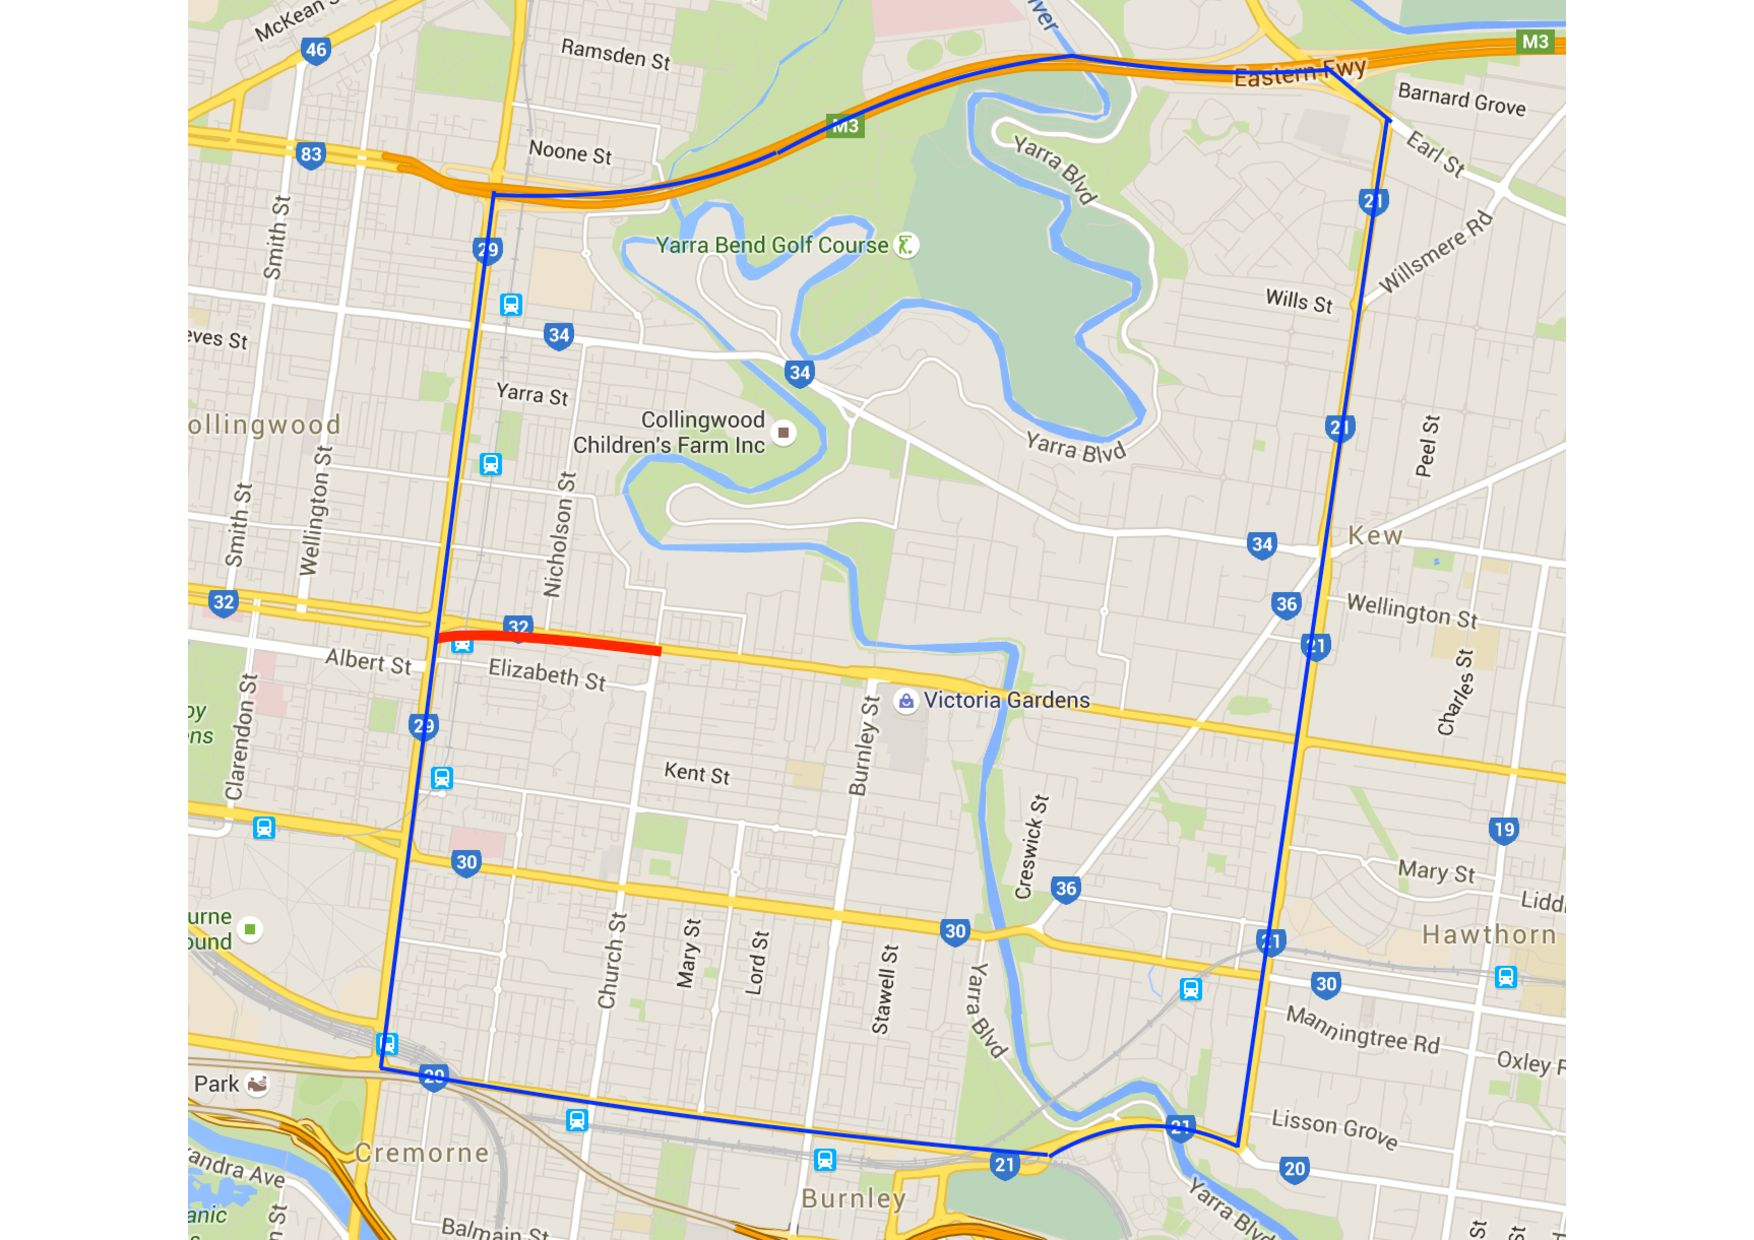
\includegraphics[width=\textwidth,height=\textheight,keepaspectratio]{Figures/experiment-region.pdf}
    \rule{35em}{0.5pt}
  \caption[Experiment traffic region]{The traffic region used in this experiment. The boundary is
   dentoed by the red line.}
  \label{fig:ExperimentRegion}
\end{figure}

\subsection{Training details}
We trained our stacked LSTM network(\ref{sec:stackedLSTMTrafficPred})

\section{Results}

For comparison purose we used the following methods that have been in used predominantly in short
term traffic prediction - Naïve, Linear regression, ARIMA, Exponential smoothing and Feedforward
neural network. In figure \ref{fig:benchmarkModels}, we present the predictions of these models
on test data. The input sequence was set to 96 observations(1 day) and the prediction was done for
next 15 minutes(1 step ahead).


\begin{figure}[h]
    \centering

    \subfloat[Linear Regression][Linear Regression]{
    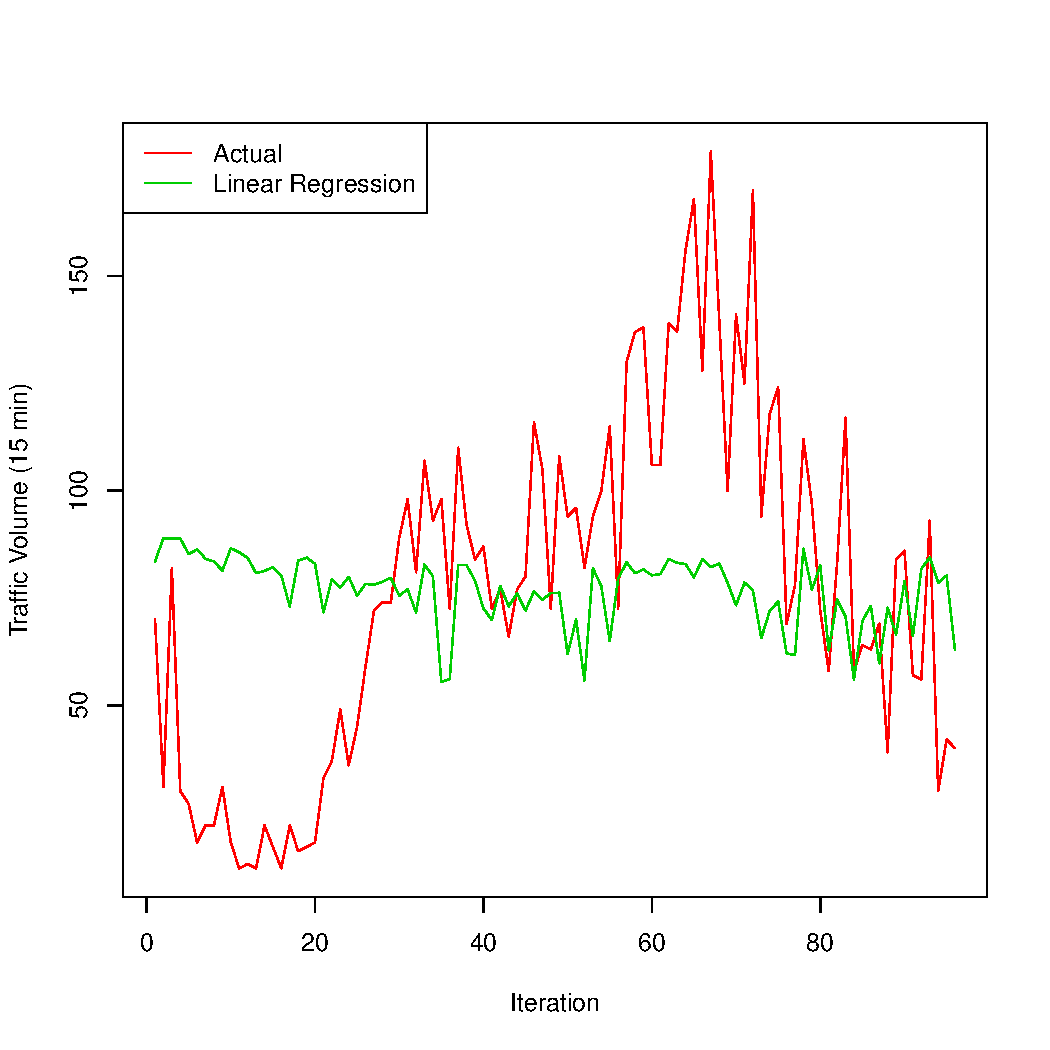
\includegraphics[width=0.4\textwidth]{Figures/linear-regression.pdf}
    \label{fig:LmActualPredicted}}
    \qquad
    \subfloat[ARIMA][ARIMA]{
    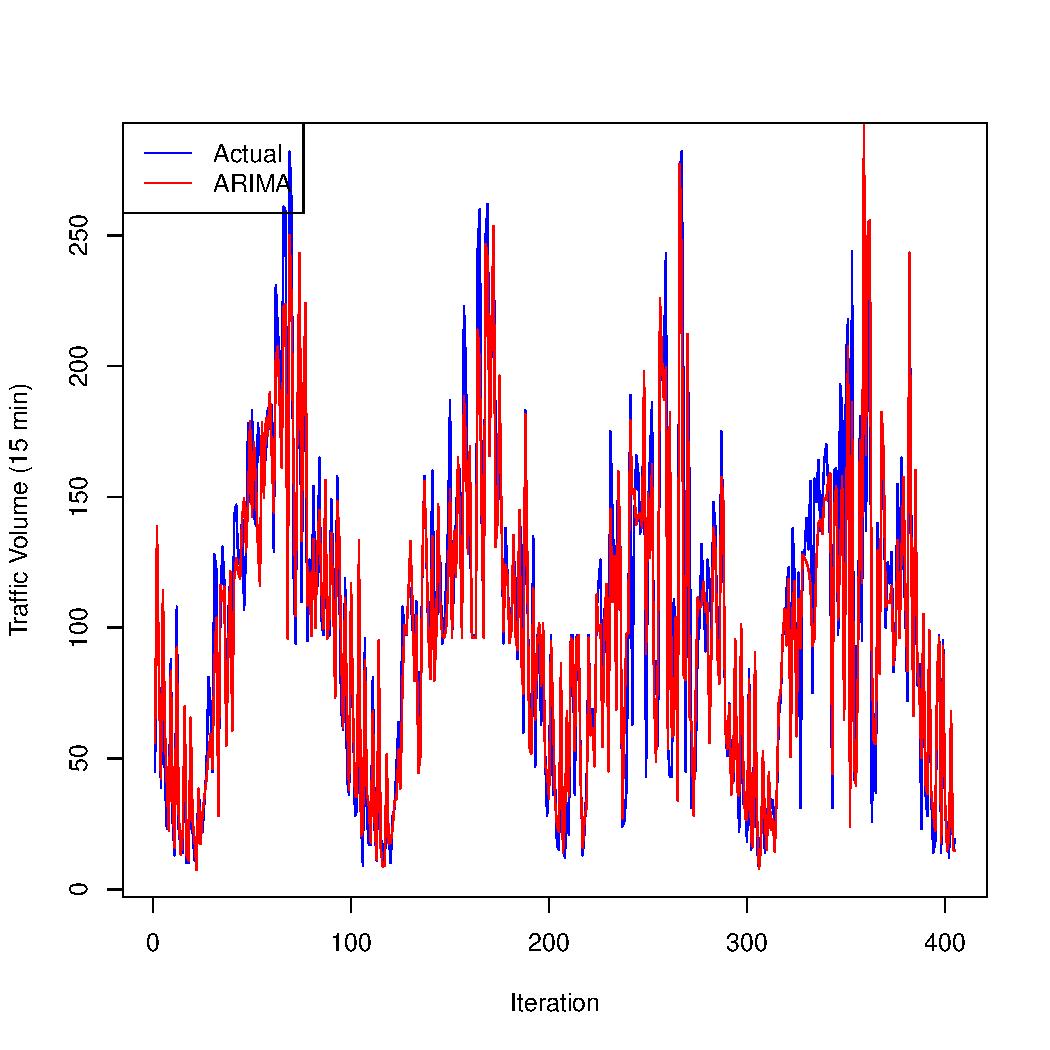
\includegraphics[width=0.4\textwidth]{Figures/arima.pdf}
    \label{fig:ArimaActualPredicted}}

    \subfloat[Exponential smoothing state space model][Exponential smoothing state space model]{
    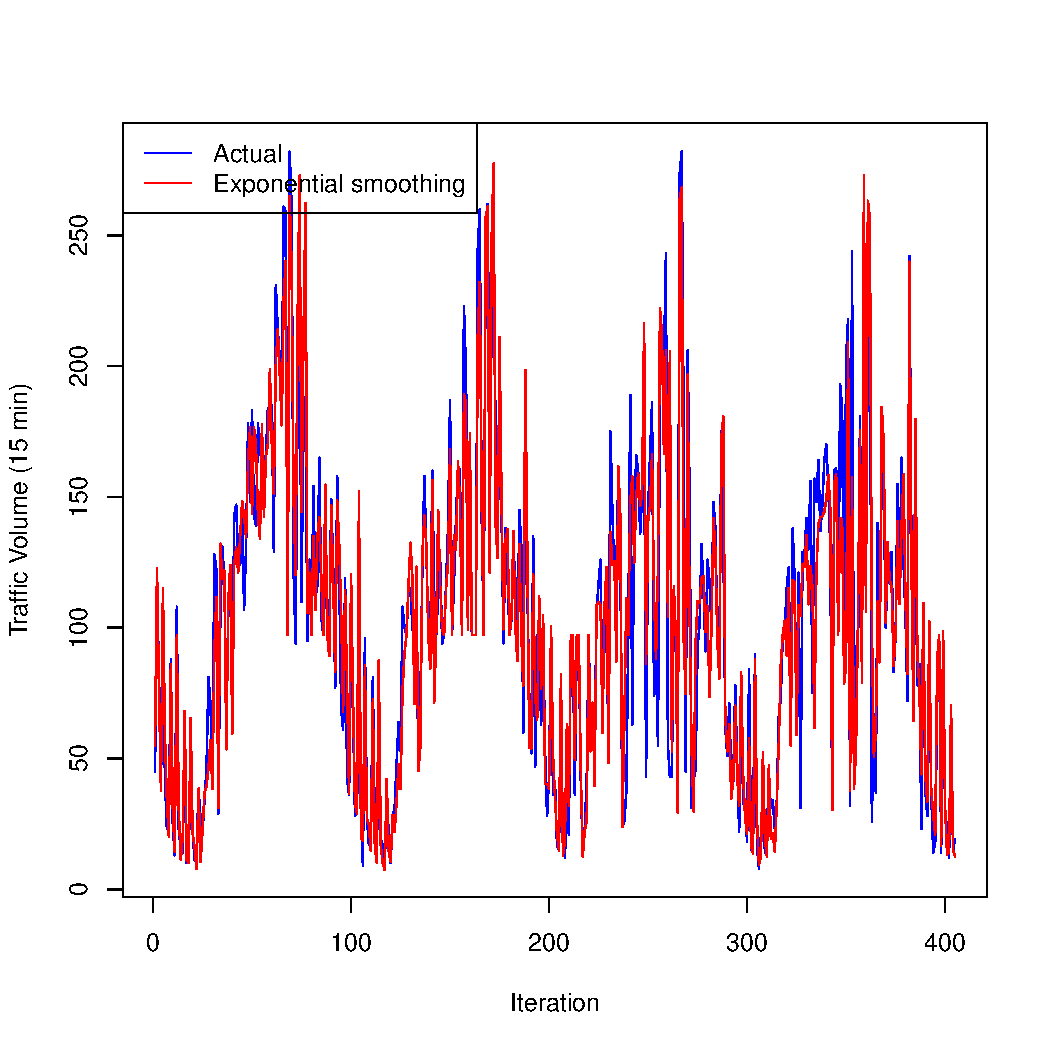
\includegraphics[width=0.4\textwidth]{Figures/exp-smoothing.pdf}
    \label{fig:etsActualPredicted}}
    \qquad
    \subfloat[BP Neural Network][BP Neural Network for time series]{
    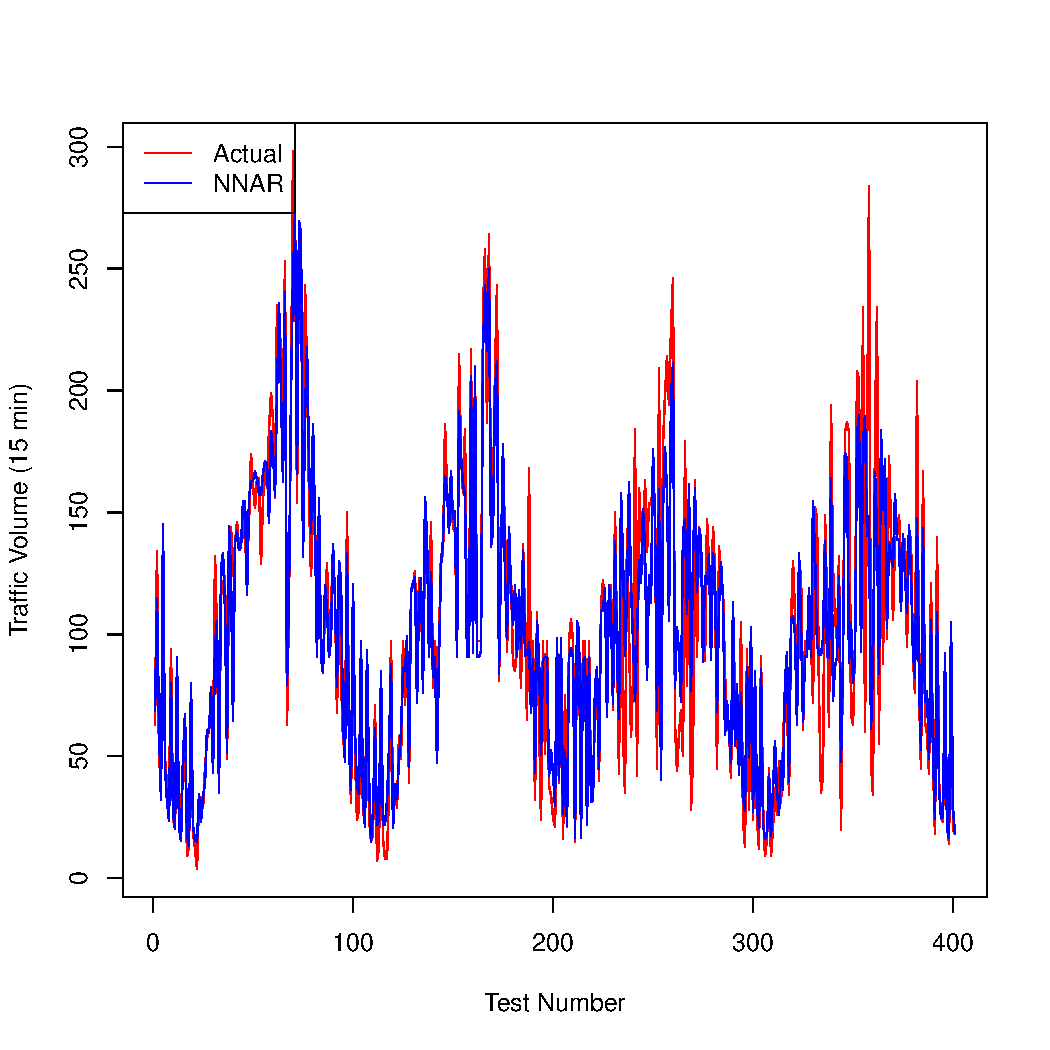
\includegraphics[width=0.4\textwidth]{Figures/nnetar.pdf}
    \label{fig:NnetarActualPredicted}}

    \caption[Acutual vs Predictions, using currently popular methods]{Acutual vs Predictions -
    linear regression, ARIMA, feed forward neural network one hidden layer and exponential
    smoothing using state space model. The models were trained on trafiic data from one homogeneous
    road segment. The plots show the actual vs predictions(15 mins) on 400 test examples, for one
    of those road segment (Nicholson street between Gertrude street and Victoria Parade).}
    \label{fig:benchmarkModels}
\end{figure}

The results of the LSTM network are shown in the figure \ref{fig:LSTMActualPredicted}

\begin{figure}[h]
    \centering

    \subfloat[Stacked LSTM - single location][Single location]{
    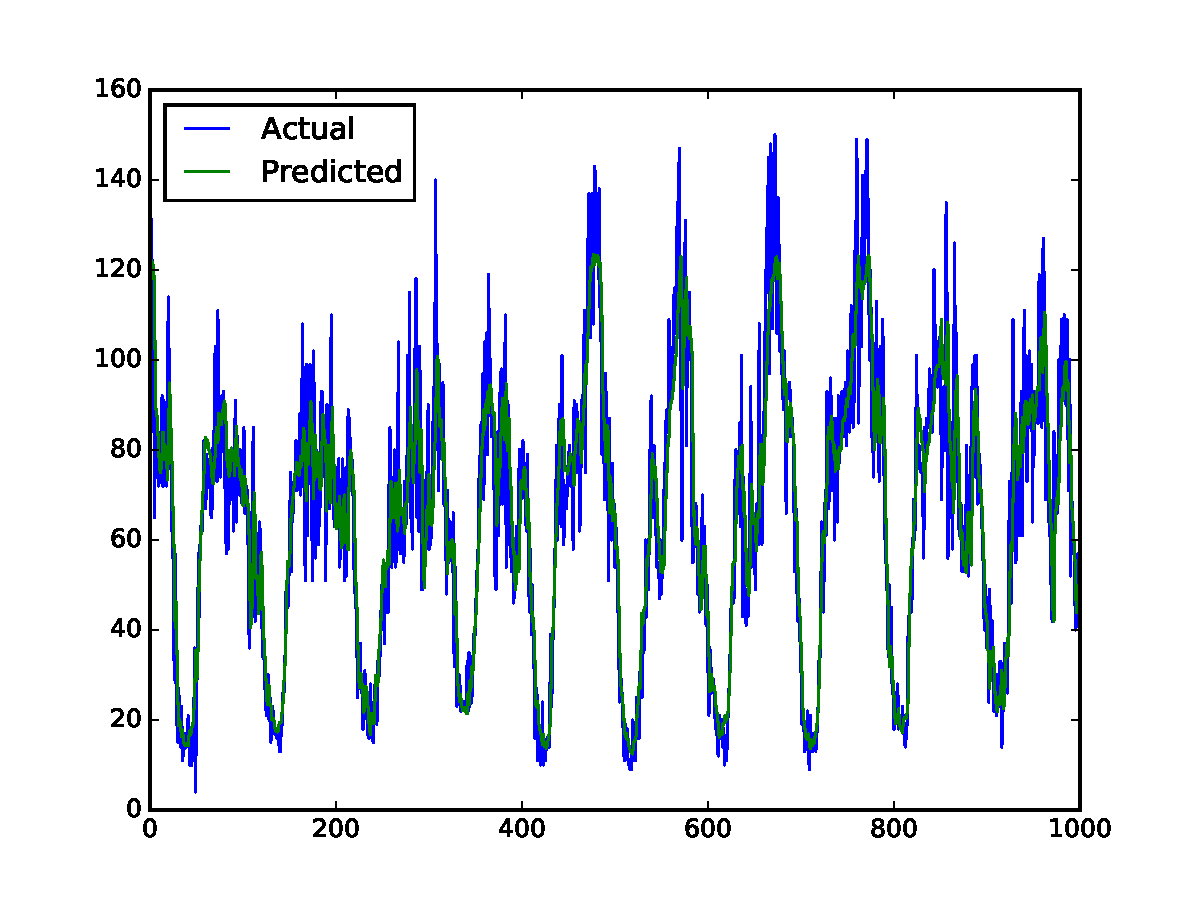
\includegraphics[width=0.4\textwidth]{Figures/lstm.pdf}
    \label{fig:LSTMActualPredicted1}}
    \qquad
    \subfloat[Stacked LSTM - multiple locations][Multiple locations]{
    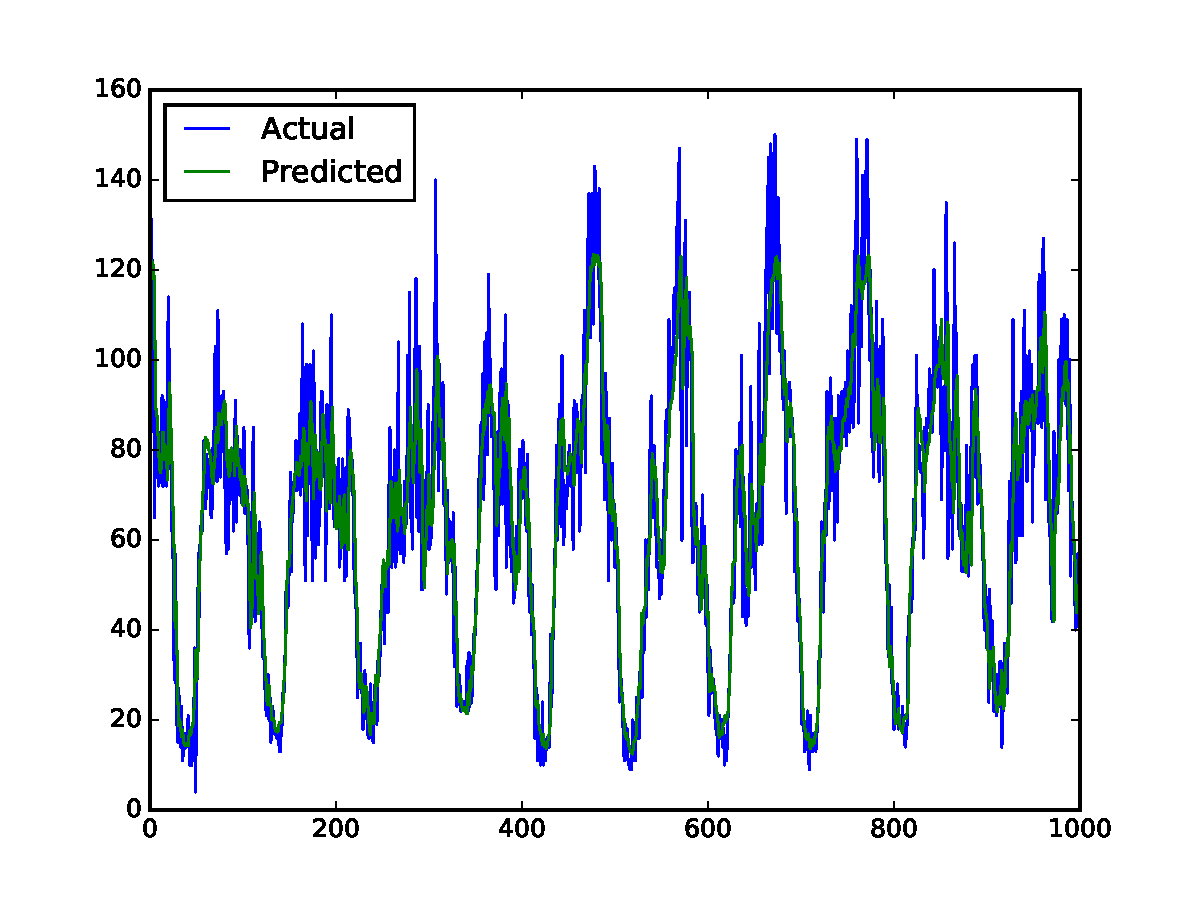
\includegraphics[width=0.4\textwidth]{Figures/lstm.pdf}
    \label{fig:LSTMActualPredicted2}}

    \caption[Acutual vs Predictions, using deep LSTM networks]{Acutual vs Predictions - The left
    figure is from the model trained using data from a single homogeneous road segment only. The
    figure in right is from the model trained on 67 homogeneous road segements in the chosen
    subnetwork(\ref{fig:ExperimentRegion}). Both the plots show the actual vs predictions(15
    mins) on 400 test examples, for one of those road segment(Nicholson street between Gertrude
    street and Victoria Parade).}
    \label{fig:LSTMActualPredicted}
\end{figure}

In table \ref{table:accuracyScores}, the performance of the LSTM network along with the compared
models are given. Several accuracy measures exist to evaluate a model. In below secions we describe
the accuracy mesures and use those to evalute our proposed model against the benchmark models.
For defining the accuracy measures let us denote $x_{i}$ be the $i^{th}$ observation and
$\hat{x}_{i}$ be the prediction of $x_{i}$.

\textbf{Scale-dependent errors}
The prediction error is simply given by $e_{i} = x_{i} - \hat{x}_{i}$, which is in the same scale
as of the original data. So accuracy measures that depend on $e_{i}$ are scale dependent and can
not be used across multiple series on different scales. The two most used scale-dependent
accuracy measures are mean absolute error and root mean squared error defined as below

    \begin{equation}
        MAE = mean(\abs{e_{i}})
    \end{equation}
    \begin{equation}
        RMSE = \sqrt{mean(e^{2}_{i})}
    \end{equation}

MAE is easy to understand and popular in usage when using a single dataset.

\textbf{Percentage errors}
Percentage errors are scale-independent and thus used across multiple datasets on different
scales. The percentage error is given by $p_{i} = 100*e_{i}/x_{i}$. The most commonly used
percentage measure is Mean Absolute Percentage Error(MAPE) which is given by the below formula
    \begin{equation}
        MAPE = mean(\abs{p_{i}})
    \end{equation}

There are however few shortccomings of the MAPE, for instance when $x_{i}$ is 0 or very large.
Another shortcoming is that they put heavier penalty on negative error values than positve error
values.

\textbf{Scaled errors}
\citet{hyndman2006another} proposed scaled errors to be used as an alternative in place of
percentage errors. The proposed Mean Absolute Scaled Error(MASE) is defined as

    \begin{equation}
        MASE = mean(\abs{q_{i}})
    \end{equation}

where
    \begin{equation}
        q_{i} = \frac{e_{i}}{\frac{1}{T-1} \displaystyle\sum_{t=2}^{T}\abs{x_{t} - x_{t-1}}}
    \end{equation}

A scaled error is less than one if it is better than the average naïve forecast computed on the
training data and vice versa.

%%
% MEAN 15 minutes traffic volume is = 104.4

%[1] "Mean Forecast..."
% 15 MINUTES
%[1] "RMSE =  48.1291966646441"
%[1] "MAE =  48.1291966646441"
%[1] "MAPE =  98.3410581401692"
%[1] "MASE =  Inf"
% 30 MINUTES

%[1] "Naive..."
% 15 MINUTES
%[1] "RMSE =  15.2469135802469"
%[1] "MAE =  15.2469135802469"
%[1] "MAPE =  21.2435033738567"
%[1] "MASE =  Inf"
% 30 MINUTES

%[1] "Linear Regression..."
% 15 MINUTES
%[1] "RMSE =  50.2963579162249"
%[1] "MAE =  50.2963579162249"
%[1] "MAPE =  97.844026487277"
%[1] "MASE =  Inf"
% 30 MINUTES

%[1] "Feedforward Neural Network....."
% 15 MINUTES
%[1] "RMSE =  19.4785975022794"
%[1] "MAE =  19.4785975022794"
%[1] "MAPE =  24.3756488596144"
%[1] "MASE =  1.30632416624528"
% 30 MINUTES

%[1] "Exponential Smoothing....."
% 15 MINUTES
%[1] "RMSE =  15.3302574006633"
%[1] "MAE =  15.3302574006633"
%[1] "MAPE =  20.680574329633"
%[1] "MASE =  1.04054865720154"
% 30 MINUTES

%[1] "ARIMA....."
% 15 MINUTES
%[1] "RMSE =  15.1000087920356"
%[1] "MAE =  15.1000087920356"
%[1] "MAPE =  21.2947271419304"
%[1] "MASE =  1.02257705105811"
% 30 MINUTES

\begin{table}
\centering
    \begin{tabular}{| l | l | l| l | l | l | l|} \hline
        Model & \multicolumn{2}{|c|}{RMSE} & \multicolumn{2}{|c|}{MAPE(\%)} & \multicolumn{2}{|c|}{MASE} \\
        & 15 mins & 30 mins & 15 mins & 30 mins & 15 mins & 30 mins \\ \hline
        Mean & 48.13 &  & 98.34 &  & Inf &  \\
        Naive & 15.25 &  & 25.24 &  & Inf &  \\
        Linear Regression & 50.30 &  & 97.84 &  & Inf &  \\
        ARIMA & 15.1 &  & 21.3 &   & 1.02 &  \\
        Eponential Smoothing & 15.33 &   & 20.68 &  & 1.04 &  \\
        Feedforward Neural Network & 19.48 &  & 24.37 &  & 1.31 &  \\
        Stacked Autoencoders &  &  &  &  &  &  \\
        Stacked LSTM &  &  &  &  &  &  \\ \hline
    \end{tabular}
    \caption[Model comparisons]{Accuracy measures - RMSE, MAPE and MASE scores for the evaluted
    models. The scores are calculated for prediction horizon of 15 and 30 minutes}
    \label{table:accuracyScores}
\end{table}